\documentclass[fleqn]{kththesis}


\usepackage{csquotes} % Recommended by biblatex
\usepackage{biblatex}
\usepackage{todonotes}
\usepackage{bytefield}
\usepackage{tikz}
\usepackage{amsmath}
\usepackage{amssymb}
\usepackage{caption}
\usepackage{enumitem}
\usepackage{verbatim}

\DeclareCaptionType{equwithcap}[][List of equations]
\captionsetup[equwithcap]{labelformat=empty}

%\usepackage[swedish]{babel}
\usetikzlibrary{shapes,arrows}
\addbibresource{references.bib} % The file containing our references, in BibTeX format
\tikzstyle{redblock} = [rectangle, rounded corners, minimum width=3cm, minimum height=1cm,text centered, draw=black, fill=red!30]
\tikzstyle{blueblock} = [rectangle, rounded corners, minimum width=3cm, minimum height=1cm,text centered, draw=black, fill=blue!30]
\tikzstyle{startstop} = [rectangle, rounded corners, minimum width=3cm, minimum height=1cm,text centered, draw=black, fill=red!30]
\tikzstyle{io} = [trapezium, trapezium left angle=70, trapezium right angle=110, minimum width=3cm, minimum height=1cm, text centered, draw=black, fill=blue!30]
\tikzstyle{process} = [rectangle, minimum width=3cm, minimum height=1cm, text centered, text width=3cm, draw=black, fill=orange!30]
\tikzstyle{decision} = [diamond, minimum width=3cm, minimum height=1cm, text centered, draw=black, fill=green!30]
\tikzstyle{arrow} = [thick,->,>=stealth]

\title{Prestudy: Formal verification of a one time pad crypto device}
\alttitle{Förstudie: Formell verifikation av en engångskryptomaskin}
\author{Adam Johansson}
\email{adajoh@kth.se}
\supervisor{Roberto Guanciale}
\examiner{Mads Dam}
\programme{Master in Computer Science}
\school{School of Computer Science and Communication}
\date{\today}


\begin{document}

% Frontmatter includes the titlepage, abstracts and table-of-contents
\frontmatter

\titlepage

%\begin{abstract}
%  Abstract goes here.
%\end{abstract}

%\begin{otherlanguage}{swedish}
%  \begin{abstract}
%    Abstrakt går här.
%  \end{abstract}
%\end{otherlanguage}


\tableofcontents


% Mainmatter is where the actual contents of the thesis goes
\mainmatter


\chapter{Introduction}

\section{Formal verification}
\paragraph{}
%TODO add reference maybe
All computer users have probably lost time or work to misbehaving software. Building bug-free programs is incredibly hard, if not impossible. Software fails even when the budget allows for rigorous testing, such as the Ariane 5 Satellite disaster, when a \$1 billion dollar prototype exploded due to software failure. In other cases, like when the Therac-25 radiation therapy machine incorrectly over-radiated patients, it has lead to actual injury and death. This project aims to produce a \emph{formally verified} crypto system employing the one time pad algorithm. 

\paragraph{}
Formal verification is the act of mathematically proving properties of hardware or software. Compared to testing or static/dynamic checking of software, formal verification is strictly stronger allowing us to prove abscence of entire classes of bugs. At least if we make (admittedly rather large) assumptions regarding the correctness of non-verified parts of the system, such as hardware. Formal verification can be done at various levels of abstraction and the level of abstraction chosen demands trust in all non-proven subsystems below that level. If formal verification is employed at the program \emph{language level} you would thus have to trust the compiler, maybe a runtime system, the operating system, hardware etc. The set of systems you rely on is sometimes referred to as the trusted computing base (TCB). % should i refer to lampson here? 
\paragraph{}
Minimizing the TCB leads to a higher assurance that the proofs produced are valid. Minimizing of the TCB can be achieved in two ways, either by proving properties at a lower abstraction level or relying on systems that already have been formally verified. 

\section{The crypto system}
\paragraph{}
The task is to formally verify correctness and other security properties, defined in this prestudy as well as during the project, of a crypto device running on simple ARM hardware. The crypto algorithm chosen for this project is one time pad. The reasoning behind using one time pad is simplicity of implementation and its proven property of \emph{perfect secrecy} \parencite{shannon_otp}. Plaintext will be received over serial port and the key will be saved on the device along with the program. The resulting ciphertext from XOR-ing the plaintext and key will be sent on a separate serial port. The aim of building this prototype is to demonstrate the power of formal verification and, in the future, investigate whether formal verification can be used to convey to a potential customer which security properties hold for a given product. 

\begin{figure}[!h]
\centering
    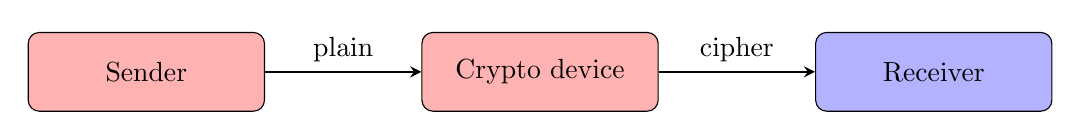
\begin{tikzpicture}[node distance=5cm]
        \node (sender) [redblock] {Sender};
        \node (cryptodev) [redblock, right of=sender] {Crypto device};
        \node (receiver) [blueblock, right of=cryptodev] {Receiver};
        
        \draw [arrow] (sender) -- node[anchor=south] {plain} (cryptodev);
        \draw [arrow] (cryptodev) -- node[anchor=south] {cipher} (receiver);
    \end{tikzpicture}
\caption{Plaintext is sent from some sender to the crypto device which in turn sends the cipher to some receiver. There is no two-way communication and blocks marked red are considered to be in a safe network.}
\label{overview}
\end{figure}



\section{Serial protocol}
\paragraph{}
In figure \ref{protomsg} protocol messages are defined. The same protocol is used whether data is plaintext or ciphertext and a message consists of two fields of 1 byte for index, refering a key block for encryption, and eight fields of 1 byte for data. \ref{indexfield} and \ref{datafield} describes the format of index fields and data fields respectively. Indices are marked with a 1 in the most significant bit (MSB) and data fields with a 0 in the MSB. This allows us to have a very simple protocol but still be able to resynchronize if a single byte is lost. 

\paragraph{}
Resynchronization can be done by first reading 10 bytes into a buffer, if the MSB of those 10 bytes do not match the pattern \texttt{1 1 0 0 0 0 0 0 0 0}, shift the buffer one byte and read one more byte until the pattern is matched. With 1 bit reserved in index fields the total number of bits possible for indexing is 14. With a key block size of 8 bytes, this means the maximum addressable key size is 128 KiB, which is sufficient for a simple prototype. 

\vspace{5mm}
\begin{figure}[!h]
\centering
    \begin{bytefield}[bitwidth=1.0em]{8}
        \bitheader{0,7,15,31} \\
        \bitbox{8}{Index[0]} & 
        \bitbox{8}{Index[1]} \\
        \bitbox{8}{Data[0]} & 
        \bitbox{8}{Data[1]} &
        \bitbox{8}{Data[2]} &
        \bitbox{8}{Data[3]} \\
        \bitbox{8}{Data[4]} &
        \bitbox{8}{Data[5]} &
        \bitbox{8}{Data[6]} &
        \bitbox{8}{Data[7]} 
    \end{bytefield}  
\caption{Protocol message with (exactly) two fields for key index and 8 fields for data.}
\label{protomsg}
\end{figure}

\begin{figure}[!h]
\centering
    \begin{bytefield}[bitwidth=1.0em]{8}
        \bitheader{0,1,2,3,4,5,6,7} \\
        \bitbox{1}{1} & 
        \bitbox{7}{Index} 
    \end{bytefield} 
\caption{Bits of the index field. Indices always have the MSB set to 1.}
\label{indexfield}
\end{figure}

\begin{figure}[!h]
\centering
    \begin{bytefield}[bitwidth=1.0em]{8}
        \bitheader{0,1,2,3,4,5,6,7} \\
        \bitbox{1}{0} & 
        \bitbox{7}{Data} 
    \end{bytefield} 
\caption{Bits of the data field. Data fields always have the MSB set to 0.}
\label{datafield}
\end{figure}
\vspace{5mm}

\paragraph{} Let $0 \leq n < 8$  denote the data index and \texttt{i} be the 14 bit key index. Let \texttt{Key[i+n]} denote the key at index \texttt{i} with offset \texttt{n} bytes. The ciphertext will be produced by \texttt{Cipher[n] := Data[n] $\oplus$ Key[i + n]} and be serialized for transport by setting the MSB of each \texttt{Cipher[n]} to 0. The index and its field identifiers will be the same as the input message.


\chapter{Literature study}

\section{One time pad}
One time pad is a symmetric cryptographic algorithm that is easy to implement and provably impossible to crack without the key. Its main drawback is that the pre-shared key must be at least as long as the plain text. The key also need to be truly random.
The encryption scheme by \textcite{shannon_otp} over a message of bits $M$ of length $l$ and a key of bits $K$ is defined below. The operator $\oplus$ is the binary XOR operator.
\begin{equation*}
\begin{split}
&M \colon \{0,1\}^l \\
&K \colon \{0,1\}^l \\
&Enc(k, m)= m \oplus k, m \in M, k \in K
\end{split}	
\end{equation*}

The definition of \emph{perfect secrecy} is, informally, that the probability of an adversary finding out the plaintext is equal with or without access to the ciphertext.  
%TODO formal definition of perfect secrecy

\section{Hardware and models}
The BBC microbit \parencite{microbit} is a widely available, well documented small computer with a 32-bit ARM Cortex M0 CPU with the ARMv6-M Thumb instruction set. It allows UART communication over USB and GPIO. Any device with sufficient amount of communication channels and an ARM processor would fit well for this project due to there being a good, well-tested model for HOL4. 
\\
The UART communication will be modelled in another thesis and that model will be integrated at the end of this project. There is a model for the ARM processor and related peripherals such as memory. It is described in detail in \parencite{trustworthy_monad} and models the fetch, encode, execute cycle with enough detail do have an instruction executed and its effects observed. It has been thoroughly tested on at least ARM Cortex M3 and ARM Cortex M8.


\section{Security issues}

\subsection{Code injection and control flow injection}
An attacker achieves code injection by leveraging bugs in applications, for example buffer overflows where input is written into the memory area after a buffer. Either that area already contains code that is supposed to be executed or the control flow of the application is manipulated to have the program execute the injected code. Control flow injection is when the attacker manipulates only the \emph{control flow graph} (CFG) (or informally, manipulates the order of execution), to execute existing code in a manner not intended by the application developer. 
\paragraph{}
An example of code injection is a \emph{buffer overflow} attack where a bug in the program allows the attacker to overwrite code segments that lie after a buffer in memory. A common countermeasure is making all executable areas of the memory read-only which prevents code injection but not necessarily control flow injection.

\subsection{Side channel attacks}
A side channel is essentially an output or input of a system that occurs as a side effect of executing the system. Examples include, but are not limited to power consumption, electromagnetic radiation, inadvertent cache leaking, timing and acoustic properties of the system. 
\paragraph{}
Side channel attacks can be mitigated, at least partially, by restricting physical access and providing special instruction sets which instructions power consumption and execution time is hard to analyze. On the software level, algorithms can add superfluous instructions to make all paths take a similar amount of time. The common goal of all mitigations of side channels is to ensure that there are no observable difference between two executions where the non-secret inputs are identical but the secret inputs are different.


%This is maybe a bit weak...
\section{Correctness}
Correctness is a property of programs and algorithms that holds if the algorithm is correct according to some form of specification.
Hoare introduced an axiomatic system to reason about correctness. The main concept of that system is the Hoare-triple, denoted as $P \{Q\} R$ where $P$ is a statement that holds before an execution, $Q$ is the program to be executed and $R$ is a statement that holds after the execution of the program $Q$. $P$ is called the \emph{precondition} and $R$ is called the \emph{postcondition}

\paragraph{}
The meaning of the notation $P \{Q\} R$ in the axiomatic system Hoare constructed relies on the assumption that the program $Q$ terminates. This reliance is captured in the notion of \emph{partial correctness}. That system was extended by \textcite{total_correctness} to add the requirement of termination in order to prove \emph{total correctness}, which is what this project mainly will be aiming for.

\subsection{Composition}
The rule of composition, as introduced by Hoare, says that if you have some triple $P_{1} Q_{1} R_{1}$ which is proven and you have another proven triple $P_{2} Q_{2} R_{2}$ where its precondition $P_{2} = R_{1}$, both program sequences together are correct given the precondition $P_{1}$. Formally:

\paragraph{}
If $\vdash P_{1} \{Q_{1} \} R_{1}$ and $\vdash R_{1} \{Q_{2}\}  R_{2}$ then  $\vdash P_{1} \{Q_{1}; Q_{2}\} R_{2}$


\section{Decompilation tool}
There are two decompilation tools available that decompile machine code into HOL4 theorems.
The first one was developed by \textcite{myreen_decompile} and was later improved by \textcite{anthony_decompile}. The latter improved version is faster but more restrictive, leading to Anthony Fox's suggestion to go with the initial decompiler of Myreen.

The actual output of the decompiler is twofold, one or several theorems of Hoare triples $\{P\} \{Q\} \{R\}$ where $P$ is a set of preconditions over state elements of the system, like the program counter, registers and their values as well as the memory state. $Q$ is a list of machine code instructions and $R$ is the postconditions defined analogously to the preconditions. The hoare triples represent a \emph{total correctness} specification. The other output of the decompiler is a high level function $f$ defined in HOL4 that describes the effects of the machine code and a precondition function $f_{pre}$ that describes which side conditions must hold before executing $f$.


%I guess this is really hard to follow, especially if one does not know anything in separation logic, but I wanted to at least explain shortly what the operator meant before giving an example.
\paragraph{}
The $\ast$-operator is the \emph{separating conjunction} operator borrowed from separation logic. The decompiler defines its $\ast$-operator over sets of system states in such a way that the operands are disjunct sets of system states. 

\paragraph{}
\textbf{Example:}

\begin{itemize}[label={}]
\item \{\verb|(r0, r1, m)| \textbf{is} $(r0, r1, m)$ $\ast$ pc \emph{p} $\ast$ $f_{pre}(r0, r1, m)$\} 
\item \emph{p}: instr1 \dots \emph{p+x}: instrX 
\item \{\verb|(r0, r1, m)| \textbf{is} $f(r0, r1, m)$ $\ast$ pc \emph{p + x}\} 
\end{itemize}

\paragraph{}
The first line in the example above are the preconditions. In informal terms, it says that we depend on two registers, \verb|r0| and \verb|r1|, the rest of the memory state is \verb|m|. Furthermore the generated precondition $f_{pre}(r0, r1, m)$ must hold and the program counter pc must have the value \emph{p}, pointing to the first instruction to be executed.

\paragraph{}
After executing all instructions, the postcondition of the generated function $f(r0, r1, m)$ must hold and the program counter points at the last instruction.

%We could add composition, frame rule etc here.

\begin{comment}
\section{Information flow analysis}
Information flow analysis is described on the language level by \parencite{sabelfeld_ifa}. It is a formalization of how information flows in a system. A variable is labeled either high (Secret) or low (Public) and the goal is to ensure that no information from a variable labeled high flows to a variable labeled low. \emph{Explicit flows} are when a variables information flows directly to another variable, for example an assignment. The label of the variable being assigned is then explicitly transferred to the new variable. \emph{Implicit flows} is when the information flow is indirect, for example if a high variable is in the condition of an if-statement and the body of the if-statement contains an assignment to a low variable.  The property of \emph{non-interference} can be informally defined (assuming determinism) either as "A change in a high input does not cause a change in low output" or "if all low inputs in two states are equal, the execution of those states are indistinguishable for an attacker". \\
One issue in cryptography is that encrypting usually takes (at least) two inputs that are labelled high and produces an output that should be labelled low. Without any other mechanics, that would be a breach of non-interference. Thus, \emph{selective declassification} is introduced, which is the ability to downgrade the security label of a variable from high to low. There is a general calculus called the spi calculus to check whether this is okay.
\end{comment}



\section{Similar work}
\paragraph{}
A garbage collector was verified by \textcite{myreen_garbage}, this verification included proofs in several layers of abstraction, using the interactive theorem prover HOL4 and the decompiler. The abstractions made higher level proofs reusable for other garbage collectors while hiding the technical details of the theorems derived by Myreens decompiler. The theorems in the lowest level of abstraction are automatically generated by the decompiler from the machine code of the implementation. Theorems higher up in the hierarchy are proven manually in HOL4. 
%TODO add examples of what the abstraction hides

\paragraph{}
\textcite{automatic_block_cipher} developed a system to automatically prove equality between implementations of block ciphers. The tool could also prove equivalence between a mathematical model and an implementation. The automatic proving was limited to algorithms that could be completely unrolled, that is, elimination of loops and recursive calls by repetition. The system used a formal model of the Java Virtual Machine (JVM) and used class files as input. 

\paragraph{}
To the authors knowledge, no formal verification of a cryptographic system has been done at the machine code level. The automatic prover of \textcite{automatic_block_cipher} requires trust in the JVM, the hardware and that the secret key is not leaked by other means. 

\begin{comment}
	\paragraph{}
	An implementation of a hypervisor was shown to correspond to a model of the same hypervisor in \parencite{mads_verification_hypervisor}. They developed a tool to translate ARMv7 assembly programs to BIL (BAP Intermediate Language), used BAP to calculate weakest precondition. To calculate the weakest precondition they had to resolve all possible assignments to indirect jumps which they solved by using an SMT solver. 
\end{comment}



%Adam: Both similar works here seem to be more about correctness properties or just showing it is equivalent to some model. I should probably find some more about proving information flow properties. The paper "Automating Information Flow Analysis of Low Level Code" seemed a bit of overkill as an approach.

\chapter{Discussion}

\section{Attacker Model}
As described in figure \ref{overview} in the introduction, the crypto device is meant for use in a protected network. Thus, the attacker model does not allow for physical access to the crypto device. Since no other programs are running in the crypto device, all side channel attacks are considered out of scope for this project. The attacker may however somehow influence the sender to send a specific input so it needs to be safe from code injection and control flow injection attacks, such as buffer overflow or buffer overread. The attacker is considered to have infinite resources to attack the resulting ciphertext.

\section{Security properties}

\subsubsection{Correctness of OTP system}
This section introduces a high level specification of the crypto system. It will later be formalized in HOL along with an optional medium level specification and the low level specification derived by the decompiler. The task in HOL will be to show equivalence (for some notion of equivalence) between these different levels. 

\paragraph{}
To start with, we define all input as some mapping between natural numbers and a list of bytes, $L_{Byte} = \mathbb{N} \rightarrow Byte$. The list of bytes can contain anything, both valid and invalid messages. In order to be correct, the crypto system needs to handle malformed input, which it does by simply ignoring anything that isn't well formed input. To begin with, we want to check that the byte headers are correct and conform to the protocol. Remember that each message consisted of 10 bytes, the first two bytes is the sequence number and the other 8 bytes is data. The most significant bit (MSB) of the sequence number must always be $1$ and the MSB of every data byte must be $0$.

\paragraph{}
We define a function that marks each start byte as true of a message where the headers of all 10 bytes are correct. This is a function from some input $I \in L_{byte}$ to a list of boolean values $L_{Bool} = \mathbb{N} \rightarrow Bool$. $I(n)$ denotes accessing the n-th element of the list I, while brackets are used to access individual bits of a byte. For example, referencing the value in the first (MSB) in byte number 5 would be $I(5)[0]$.


\begin{equation*}
\varphi_{start}(I) \colon L_{Byte} \rightarrow L_{Bool}
\end{equation*}
\begin{equation*}
\varphi_{start}(I) = \lambda k .\Bigg(
(I(k)[0], \dots ,I(k+9)[0]) = 
(1,1,0,0,0,0,0,0,0,0)\Bigg)
\end{equation*}
	
\paragraph{}
So far we only have a function that marks the starting byte of a valid (in terms of byte headers) protocol message. In the next step, we use that function to find all the bytes that are part of a valid protocol message. Again, the input is defined by $I \in L_{Byte}$. The main idea here is to find the starting byte $k'$ for every byte. 
\begin{equation*}
	\varphi_{msg}(I) \colon L_{Byte} \rightarrow L_{Bool}
\end{equation*}
\begin{equation*}
	\varphi_{msg}(I) = \lambda k .\Bigg(
	\exists k' . k-10 < k' \leq k \land \varphi_{start}(I))[k'] \Bigg)
\end{equation*}

Now that we know which bytes that are part of a protocol message with valid headers we can throw away invalid input. We make use of a standard filter function $\varPi$ that takes a list of elements and a list of booleans and returns the sub list of elements (in order) that are marked true at their corresponding index in the list of booleans. We call the resulting list $V$.

\begin{equation*}
V = \varPi(I, \varphi_{msg}(I))
\end{equation*}

To have something more easy to reason about, we now introduce a type for messages as well as a function that generates such a list for us. 

\begin{equation*}
L_{msg} = N \rightarrow Byte^{10}
\end{equation*}
\begin{equation*}
M \colon L_{Byte} \rightarrow L_{msg}
\end{equation*}
\begin{equation*}
M(V) = \lambda k \Bigg( V(10k); V(10k+1); \dots ;V(10k+9)
\Bigg)
\end{equation*}

\paragraph{}
Reading the sequence number from a message is rather straightforward. Take the 7 bits of the first byte of a message, bitshift 7 steps to the left and do bitwise OR (|) with the 7 bits of the second byte of a message.

\begin{equation*}
	seq(m) = (m[0][1:7] \cdot 2^7) | m[1][1:7]
\end{equation*}

\paragraph{}
Removing messages that have a sequence number less than some constant $MAX$.

\begin{equation*}
	\varphi_{MAX}(M) = \lambda k . \Bigg(
		seq(V(k)) < MAX	
	\Bigg)
\end{equation*}

\begin{equation*}
	M_{MAX} = \varPi(M, \varphi_{MAX}(M))
\end{equation*}

\paragraph{}
We want to get rid of messages which sequence number is out of sequence, that is, if its sequence number is larger than the largest accepted so far.
%TODO add examples and more describing text
\begin{equation*}
\begin{split}
	\varphi_{seq} = \lambda k . \Bigg( &(k=0) \lor \\
	& \exists k'. (k' < k \land  \\
	&\phantom{==}\, M_{seq}[k'] \land \\
	&\phantom{==}\, \forall t. (k' < t < k \land \neg M_{seq}[t]) \land \\
	&\phantom{==}\, seq(M_{MAX}[k']) < seq(M_{MAX}[k])) \Bigg)
\end{split}
\end{equation*}

This is the most complicated function so far, so lets break it down. The term $(k=0)$ is our base case for this function. For the very first message out of $M_{MAX}$, its sequence number will trivially be the largest we've seen so far, thus it evaluates to \emph{true}. The existential quantifier says that there must exist some $k' < k$ such that it its sequence number is valid, that is, $M_seq[k']$ holds. Additionally, we say that for all $t$ in between that $k'$ and out current $k$, $M_seq[t]$ does \emph{not} hold. Thus $seq({MAX}[k'])$ must be the largest accepted sequence number so far. If $seq({MAX}[k])$ is strictly larger, the whole expression evaluates to \emph{true}, otherwise, $seq({MAX}[k])$ can't be part of a monotonically increasing sequence number and the expression evaluate to \emph{false}.

\paragraph{}
Preparing for the actual encryption step, we need to be able to resolve a key. In one time pad we need a unique key for each message. These are indexed with the sequence number, pointing to a block of 8 bytes of a constant KEY. 
\begin{equation*}
key(seq) = KEY[seq*8]
\end{equation*}

\paragraph{}
TODO the rest is much easier, but will leave it for now.


\begin{comment}
\subsubsection{Non-interference and leaking of data}
Looking at above definitions, if we have equivalence of the code to the model above, we need not consider non-interference for $f$ or those functions that only take public input. Proving that equivalence for some notion of equivalence may however still require such properties to be shown. A first draft of such properties follow below:

\paragraph{}
Let $R_{i}$ be the i-th memory mapped register and let $READ(R_{i})$ and $WRITE(R_{i})$ denote generalized read and write events to these registers. Then let $R_{in}$ and $R_{out}$ denote the memory mapped registers used for input and output respectively according to the specification.

\paragraph{}
The property of unidirectionality:
$$R_{in} \neq R_{out}$$

\paragraph{}
Single input property:
$$READ(R_{i}) \implies i = in$$

\paragraph{}
Single output property:
$$WRITE(R_{i}) \implies i = out$$

\paragraph{}
No output property:
$$\neg WRITE(R_{i})$$

\end{comment}

\subsubsection{Code injection and control flow injection}
Freedom from code injection and control flow injection follow from correctness, assume that a program $P$ is correct, implying that for all inputs it produce a specific output. Code injection implies that an attacker may send some input and have the device execute arbitrary code to have the device behave outside of its specification. But that would mean correctness doesn't hold for program $P$. Thus, a correct program is free from code injection. A similar argument can be made about control flow injection.

\subsubsection{Side channel attacks}
While the attacker model does not allow the attacker physical access to the device nor the sender, timing and power measurements attacks are impossible. Electromagnetic or audiobased attacks can also be mitigated by physical constraints. It would however, in the future, be interesting to extend the attacker model and prove the crypto device free from sidechannel attacks. 

\subsubsection{Non-interference with UART driver}
Proving the UART driver correct will be done after the UART is modelled in a separate thesis. The UART driver model will provide an interface that accepts a theorem of non-interference.

\section{Choice of method}
\paragraph{}
A stated goals of this project is to minimize the amount of software we trust in order to produce proofs that are relatively easy to understand and validate for a third party. By using Myreens decompiler \parencite{myreen_decompile}, trusting the compiler is not necessary, the third party could potentially run the proof scripts themselves on a provided binary and see which security properties still hold for that binary.  If this project were to use language level formal verification we would need to trust at least a compiler, which is contrary to the goal of minimizing the Trusted Computing Base and the implementation would be vulnerable to attacks targeting the compiler.
\paragraph{}
Ideally the theorems should be as human readable as possible, so that a third party can actually understand what is proven. This property can be achieved using any of the approaches described in the similar work section and is essentially done the same way, by abstracting away technical details and trying to provide higher level theorems. How many layers of abstraction that would be needed and if that level of abstraction can actually lead to a third party understanding the theorems without extensive knowledge of HOL4 remains to be investigated during the project.
\\
Essentially, this leads to a choice of method similar to that of \textcite{myreen_garbage} in his proofs about the garbage collector.

\section{Assumptions}
One of the assumptions that have been identified at this point is that the key is truly random. That is, each possible key is chosen with the same probability $p$. This is very important for the one-time pad as described in \textcite{shannon_otp}, without this assumption, the proof of \emph{total secrecy} would be impossible.
\paragraph{}
Additionally quite a lot of assumptions about the hardware and the model are made. For example, we assume that the ARM model is correct and correctly models an ARM Cortex M0 CPU, we assume that there are no hardware trojans in other peripheral hardware with DMA. Initially, we will also assume that the UART is correct, modelling UART and optionally providing a software implementation of UART will be the topic of another master thesis, the work of which will be merged with this project if possible.


\section{Evaluation of results}
The results of this project are the produced theorems and a working prototype. A proper evaluation of the theorems should include a section describing which assumptions that were made and what parts of the system we trust such that a reader can themselves get an insight into the strength of those theorems and the security properties they represent. The method can also be compared to other verification projects in cryptography by comparing assumptions.

\paragraph{}
Secondary result is a machinecheckable proof. Evaluation here is a bit less interesting, either the proof works or not.
\paragraph{}
Tertiary results are the proof scripts themselves, evaluation here is trickier since good properties could include reusability, understandability of code etc, which are all rather subjective properties.
\paragraph{}
The last result is that of the prototype. It will be considered successful if it is working and it is possible (with the help of simple helper programs) to send a message on one compute, have the prototype encrypt it and on a second computer be able to decrypt the message.

\section{Trust and limitation of method}
We trust the bootloader and the tools used, like the HOL4 kernel and that the ARM model is true to reality. Additionally, we have a high level of trust in the hardware. There is however no trust in the code of the implementation itself, in the compiler or any operating system.

\section{Limitations of the prototype}
The implementation will likely not be very useable in practice, there is no way to change or update the key, issues indexing plaintext and ciphertext limits the amount of total messages we can send. The resulting ciphertext isn't verified for integrity, that is, detecting modifications of the produced ciphertext is not possible without the user adding MAC or checksums in the message itself. OTP provides no authentication out of the box, so there is no guarantee that a sent message is actually sent by an authorized user unless implemented in the message.


\section{The future}
Relaxing the assumption that the attacker has no physical access would give a more reasonable attacker model and necessitate proving abscence of side channel attacks on power consumption or timing. Another venue to explore is to switch from UART, which is a bidirectional type of communication hardware to a proper data diode solution. One time pad, despite its feature of \emph{perfect secrecy}, still is not a very useable encryption scheme due to the size of the key. Looking into other symmetric encryption algorithms would put this prototype closer to a working product. Additionally, adding checksums to the protocol will increase reliability.

\section{Time plan}
\begin{enumerate}
\item Milestone 1 – end of January 
  \begin{enumerate}
      \item Prestudy complete
  \end{enumerate}
\item Milestone 2 – end of February
  \begin{enumerate}
      \item C implementation finished
      \item Decompilation of implementation
      \item Eventually, extensions to the decompiler to achieve above point
  \end{enumerate}
  \item Milestone 4 - 15th February - 15th March
  \begin{enumerate}
      \item Protocol specification formalized in HOL
  \end{enumerate}
  \item Milestone 5 – end of April
  \begin{enumerate}
      \item Code verification complete in HOL4
      \item Correctness proof
      \item Non-interference proofs
      \item Necessary abstractions in the proofs
  \end{enumerate}
\item Milestone 6 – end of May
  \begin{enumerate}
      \item Delivery of Thesis report
      \item Integration with UART project finished
      \item Delivery of HOL scripts with UART integeration
  \end{enumerate}
\end{enumerate}






\printbibliography[heading=bibintoc]

\appendix


\end{document}